\newpage
\section{Stratégie du point de vue du \textsl{Responsable des stocks}}
\label{sec:stocks}

Le responsable des stocks cherche à minimiser la contenance du stock,
\textsl{i.e.} le nombre de produits entreposés ajouté à la quantité de
matières premières. Aucune contrainte particulière n'est ajoutée mais la
recherche de l'optimum se fait sous les contraintes définies précédemment.

\subsection{Modélisation}
Soit $Stock(n_{i})$ le nombre d'unités de stock nécessaires pour stocker les
produits fabriqués et les matières premières nécessaires.\\
Cette fonction est évidemment la somme des produits fabriqués et de la quantité de matières
premières nécessaire à leur fabrication.\\
~\\
Supposons qu'\textbf{un produit fabriqué correspond à une unité de stock.}\\
~\\
Ainsi, soient :
\begin{itemize}
	\item $n_{i}$ la quantité de produits usinés (pour chaque produit $i$)
	\item $Q_{j,i}$ la quantité de matière première par produit pour chaque produit $i$ et chaque matière première $j$.
\end{itemize}
~\\
Alors :
\begin{equation}
	Stock(n) = \sum_{i} (n_{i} + n_{i} \times \sum_{j} Q_{j,i})
\end{equation}

La représentation matricielle de cette fonction sera alors :

\begin{equation}
	M_S = \begin{pmatrix}
		1 & 1 & 1 & 1 & 1 & 1
	\end{pmatrix} + (
	\begin{pmatrix}
		1 & 1 & 1
	\end{pmatrix}
	\times Q)
\end{equation}

\subsection{Stratégie adoptée}
Un résultat trivial est de ne fabriquer aucun produit :
\begin{equation}
    \begin{pmatrix}
	0 \\ 0 \\ 0 \\ 0 \\ 0 \\ 0
    \end{pmatrix}
\end{equation}

En effet, en l'absence de production, aucun stock n'est nécessaire. Ce résultat
n'est pas satisfaisant.\\
Nous allons donc nous intéresser à un second critère : \textbf{les bénéfices de l'entreprise}.\\
Pour ce faire, nous allons nous utiliser les résultats obtenus en imposant un minimum de bénéfices.\\
En réalisant les calculs sur plusieurs échelons, nous obtenons un résultat linéaire par morceaux. Le
raisonnement adopté est similaire à celui développé dans la section \ref{sec:monocrit}.

\begin{figure}[!ht]
	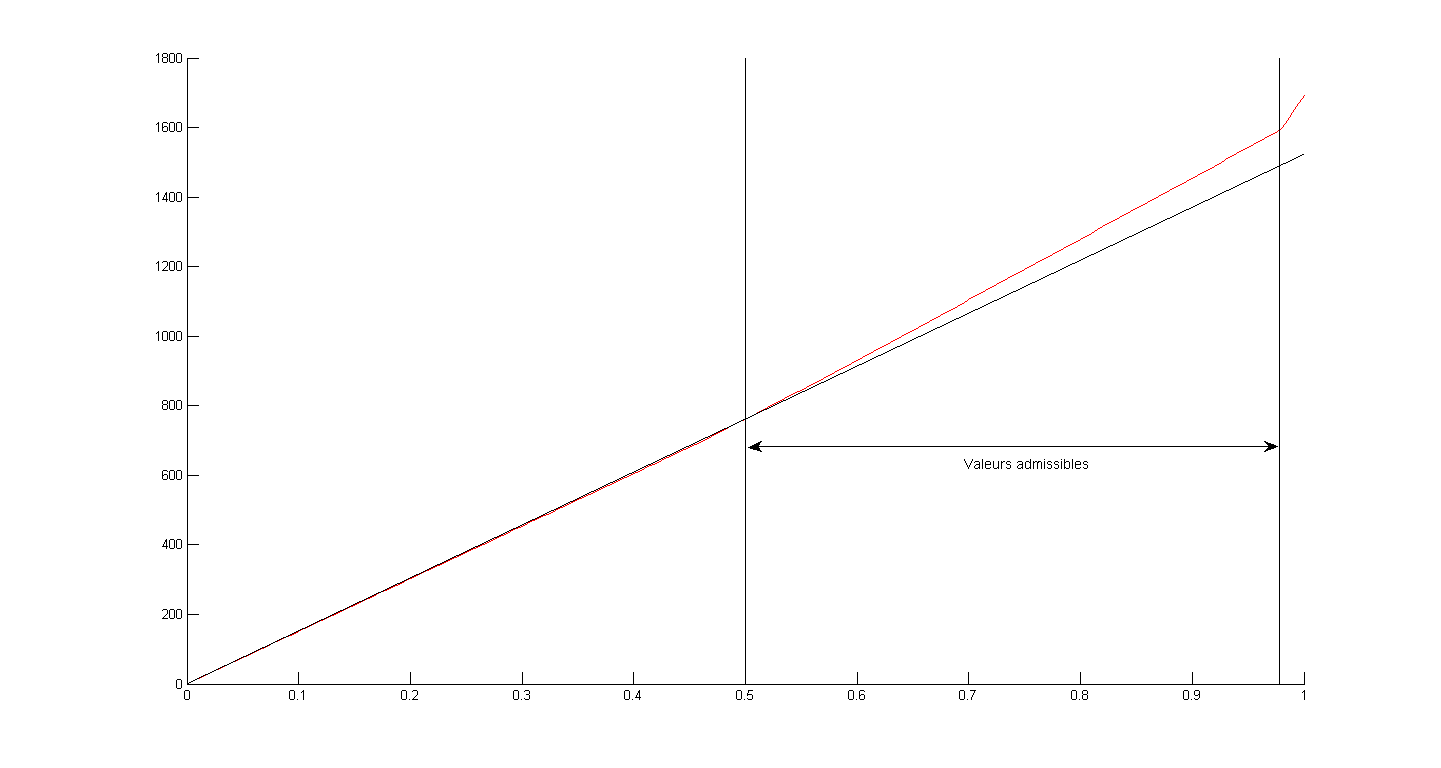
\includegraphics[width=\textwidth]{graphe_resp_stocks.png}
	\caption{Graphe de l'évolution des stocks en fonction du bénéfice}
\end{figure}

\subsubsection{Interprétation} 
De nombreuses valeurs sont équivalentes mathématiquement parlant et ne peuvent pas vraiment être départagées. 
Les choix possibles se situent dans la deuxième partie de la courbe :
\begin{itemize}
	\item En dessous, les bénéfices sont trop bas.
	\item Au dessus, les besoins de stockage augmentent beaucoup plus que les bénéfices. Nous perdons alors de vu notre
	objectif initial, \textsl{i.e.} avoir le moins de stock possible.
\end{itemize}

Nous obtenons donc une valeur comprise entre 50\% et 98\% de bénéfices. 
Pour 75\% du bénéfice maximum, nous obtenons le nombre de produits suivants :

\begin{equation}
\begin{pmatrix}
1,91903382074088 \times 10^{-10} \\
2,63753463514149 \times 10^{-10} \\ 
1,89174897968769 \times 10^{-10} \\
1,23691279441118 \times 10^{-10} \\ 
124,634235411818 \\
142,146305832495 
\end{pmatrix}
\end{equation}

\begin{center}
	\fbox{\textbf{Soit une quantité d'unités en stock de 1191,75640039347.}}
\end{center}
~\\
Cette étude de cas nous rappelle les limite d'une stratégie basée sur l'analyse d'un seul critère. En effet, 
en l'absence de contraintes assez fortes, le problème devient \og indécidable\fg mathématiquement.

C'est pourquoi nous allons combiner les 4 études réalisées pour affiner nos stratégies et obtenir une solution : 
\begin{itemize}
	\item Mathématiquement claire
	\item Respectant un ensemble de contraintes plus grand, et par conséquent qui se concentre plus sur les
	contraintes propres à l'entreprise \textbf{Optim}.
\end{itemize}
